\section{Bosques Aleatorios '\textit{Random Forests}'}
\label{resultados:rf}

\subsection{Características de los conjuntos de datos a analizar}
\label{resultados:rf_caracteristicas}
Al realizar las mismas transformaciones que para el caso de \hyperref[resultados:knn_caracteristicas]{K-NN}, las características de los conjuntos de datos son las mismas.

\subsection{(Caso de estudio 1) Resultados del entrenamiento con el Conjunto de datos solo con atributo utilidad definido y escogiendo los atributos que nos ha indicado como relevantes el \hyperref[result:pca_case2]{caso de estudio 2} del PCA}

\paragraph{}
Para realizar el entrenamiento y posterior validación del modelo de Bosques Aleatorios '\textit{Random Forests}' es necesario detectar antes a partir de que número de arboles podemos considerar que estos dan el valor a predecir correcto. Es lógico pensar que cuantos más arboles refuercen la decisión, más acertada sera esta pero, lo que hay que medir es, hasta que punto merece la pena seguir 'preguntando' si un registro es clasificado en un grupo u otro.

\paragraph{}
Esto es debido a que el modelo de Bosques Aleatorios '\textit{Random Forests}'\cite{ref:rf_def} genera versiones diferentes del conjunto de entrenamiento usando muestreo con reemplazo (\textit{bagging}\cite{ref:rf_bagging}). Esto significa que, durante el proceso de construcción de cada árbol de decisión, se selecciona aleatoriamente un subconjunto de las variables del conjunto de datos, dando opciones a variables que normalmente quedarían eclipsadas por otras que tengan mayor relevancia. Al tener un conjunto de datos con muy pocos atributos, tener un número elevado de arboles a preguntar hará que muchas veces se pregunte a arboles repetidos por lo que hay que valorar hasta que punto merece la pena seguir preguntando.

\paragraph{}
Para realizar este estudio ejecutaremos el modelo con diferentes valores de la variable \textit{n\_estimators}\cite{ref:rf_random_forest_classifier} (número de arboles en el bosque) y contrastaremos que porcentaje de acierto tiene el modelo con un subconjunto del propio conjunto de datos que conocemos su valor final. Como podemos ver en la figura \ref{rfTrainCase1}, el valor más optimo del \textbf{estimador es 40}, con un \textbf{porcentaje de acierto del 61\%}. Puede consultar el código para la realización de estos entrenamientos en el anexo (\nameref{anx05:rf1}).

\paragraph{}
Si mostramos la matriz de confusión\cite{ref:confusion_matrix} (figura \ref{rfCMCase1}) para poder ver que porcentaje de aciertos tiene el modelo con el conjunto de test, vemos que tiene un \textbf{porcentaje de aciertos bastante bajo} llegando a rozar la aleatoriedad.

\begin{figure}[!htb]
    \begin{subfigure}[b]{0.45\linewidth}
    	\centering
	    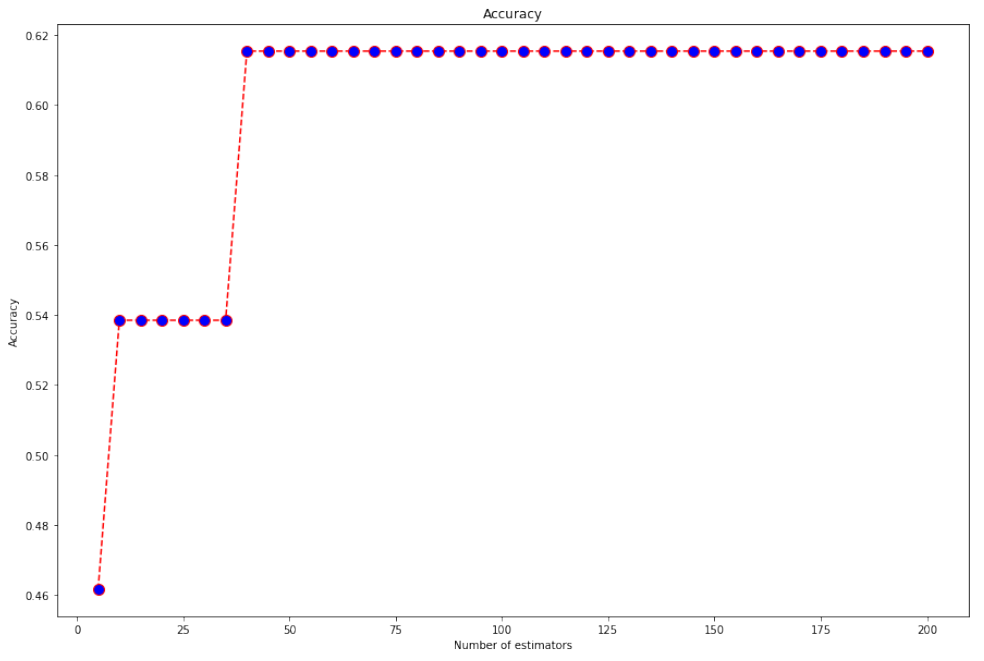
\includegraphics[width=0.9\textwidth]{images/resultados_rf_ent_conjunto1.png}
    	\caption{Calculo del valor n\_estimators para el caso de estudio 1.}
		\label{rfTrainCase1}
	\end{subfigure}
	\begin{subfigure}[b]{0.45\linewidth} 
		\centering
		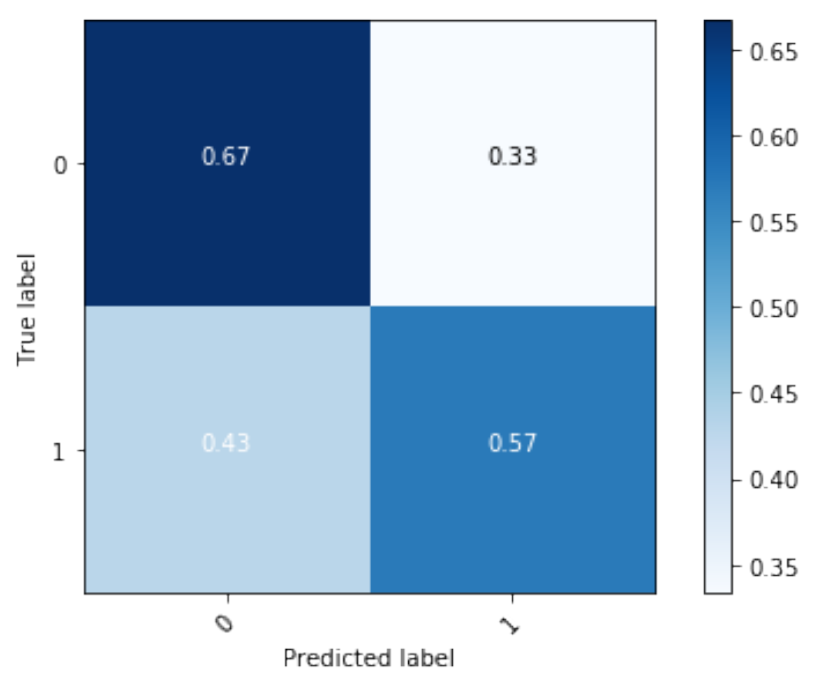
\includegraphics[width=0.7\textwidth]{images/resultados_rf_cm_conjunto1.png}
		\caption{Matriz de confusión para el modelo Random Forest en el caso de estudio 1.}
		\label{rfCMCase1}
	\end{subfigure}
	\caption{Modelo Random Forest en el caso de estudio 1.}
	\label{rfCase1}
\end{figure}

\subsection{(Caso de estudio 2) Conjunto de datos solo con atributo utilidad definido, añadiendo el mes y año del artículo, eliminando los atributos \textit{gender} y artículo y expandiendo el atributo \textit{respuesta.pubmed\_keys}. También escogemos solo los atributos que nos ha indicado como relevantes el \hyperref[result:pca_case3]{caso de estudio 3} del PCA}

\paragraph{}
Igual que en el caso anterior, realizaremos el estudio para detectar a partir de que número de \textit{n\_estimators}\cite{ref:rf_random_forest_classifier} (número de arboles en el bosque) podemos dar por supuesto que el resultado es de un grupo u otro. A diferencia del caso anterior, podemos ver en la figura \ref{rfTrainCase2}, el valor más optimo del \textbf{estimador es 10}, con un \textbf{porcentaje de acierto del 89\%}. Puede consultar el código para la realización de estos entrenamientos en el anexo (\nameref{anx05:rf2}).

\paragraph{}
Si mostramos la matriz de confusión\cite{ref:confusion_matrix} (figura \ref{rfCMCase2}) para poder ver que porcentaje de aciertos tiene el modelo con el conjunto de test, vemos que tiene un \textbf{porcentaje de aciertos bastante aceptable}.

\begin{figure}[!htb]
    \begin{subfigure}[b]{0.45\linewidth}
    	\centering
	    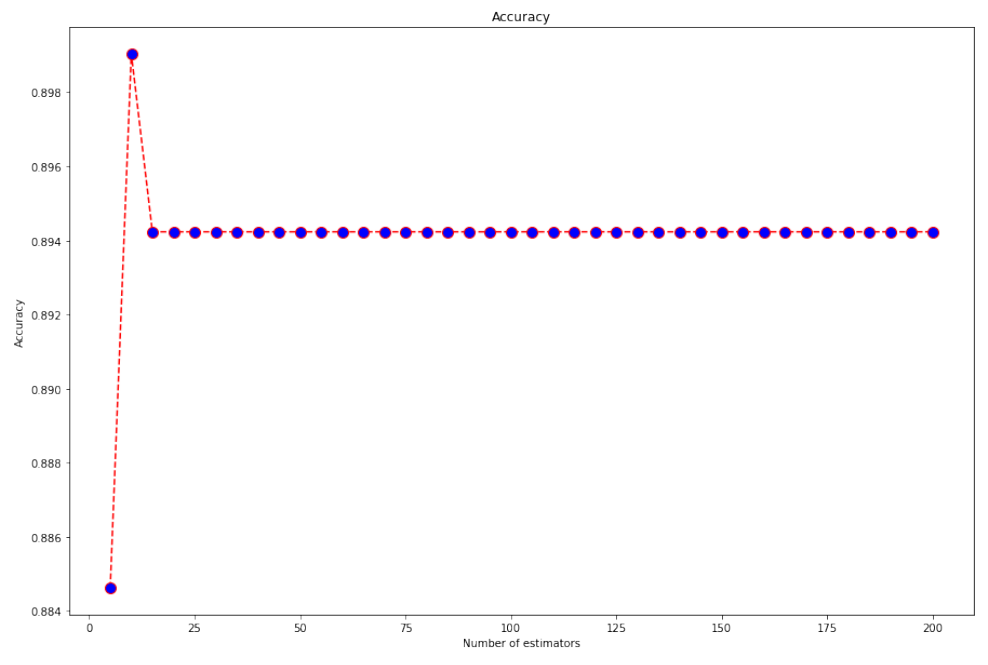
\includegraphics[width=0.9\textwidth]{images/resultados_rf_ent_conjunto2.png}
    	\caption{Calculo del valor n\_estimators para el caso de estudio 2.}
		\label{rfTrainCase2}
	\end{subfigure}
	\begin{subfigure}[b]{0.45\linewidth} 
		\centering
		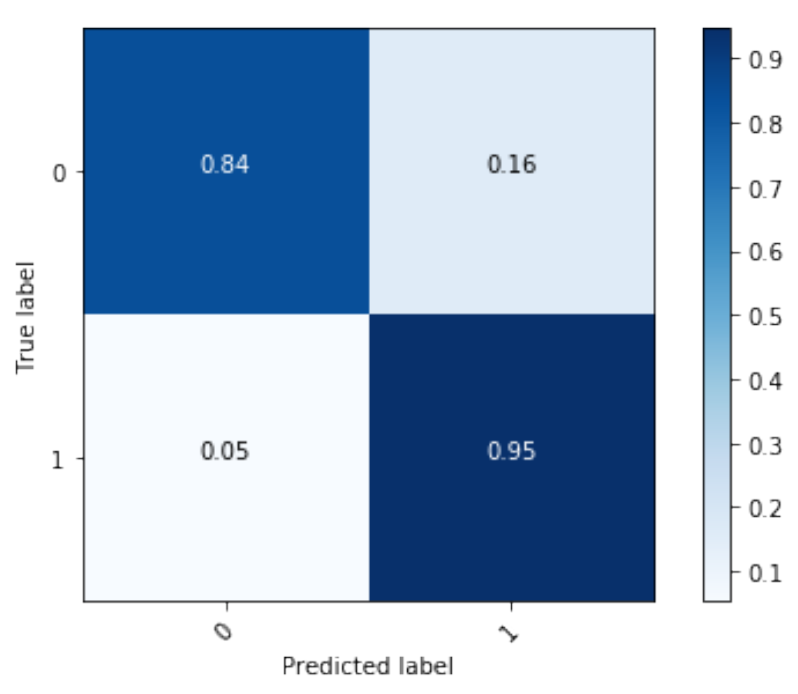
\includegraphics[width=0.7\textwidth]{images/resultados_rf_cm_conjunto2.png}
		\caption{Matriz de confusión para el modelo Random Forest en el caso de estudio 2.}
		\label{rfCMCase2}
	\end{subfigure}
	\caption{Modelo Random Forest en el caso de estudio 2.}
	\label{rfCase2}
\end{figure}

\subsection{Conclusiones del modelo de Regresión Logística}
\label{resultados:rf_conclusiones}

\paragraph{}
En este caso, podemos apreciar que el \textbf{caso 2 se ajusta a unos resultados aceptables} ya que esta lo suficientemente ajustado para que de resultados razonables sin estar sobreajustado\cite{ref:knn_overfiting}. Por lo que recomendamos al cliente como posible modelo final el modelo de Bosques Aleatorios '\textit{Random Forests}' aplicando las transformaciones al conjunto de datos realizado en el caso de estudio 2.
